\documentclass[nonacm, acmsmall]{acmart}
% Tip: add "review" to the options above to get line numbers while drafting.

\setcopyright{none}
\citestyle{acmauthoryear}

\usepackage[T1]{fontenc}
\usepackage[utf8]{inputenc}
\usepackage{booktabs}
\usepackage{graphicx}
\usepackage{listings}
\usepackage{color}
\usepackage{cleveref}

\graphicspath{{figures/}}

% Listings: JPAMB cases are Java.
\lstset{language=Java, basicstyle=\ttfamily\small, columns=fullflexible,
  keepspaces=true, numbers=left, numberstyle=\tiny, frame=tb}
\crefname{lstlisting}{listing}{listings}
\Crefname{lstlisting}{Listing}{Listings}

% Shared macros (keep all \newcommand's here, not in the sections).
\newcommand\jpamb{\textsc{JPAMB}}
\newcommand\set[1]{\left\{#1\right\}}
\newcommand\todo[1]{\textcolor{red}{\textbf{TODO:} #1}}

% ---------------------------------------------------------------------------
\title{TODO: Project Title}

\author{Deniz Isikli}
\email{s215818@dtu.dk}
\author{Cristina Semikina}
\email{s260209@dtu.dk}
\author{Krish Devendra Waghresha}
\email{s252788@dtu.dk}
\affiliation{%
  \institution{DTU Compute - Group XX}
  \city{Kgs. Lyngby}
  \country{Denmark}}

\begin{abstract}
% Abstract: a short description of the paper (~150-200 words).
Code written with AI assistance is often larger and more defensive than it needs to be, so
developers simplify it with edits that should preserve its behaviour. Such an edit is only
useful if it is reliable. Tests rarely reach the single input on which an edit is wrong. An
SMT query over two whole methods returns one yes or no answer, and a loop-free symbolic
encoding returns no answer once the methods contain loops. We present a checker that decides the question per
\emph{region} of the input space. It analyses the original and the edited JVM method
separately with an interval abstract interpreter on a box of inputs. Sound verdict rules turn
the two outcome sets into \pres{}, \chg{} or \unk{} for the whole box. We split undecided
boxes at the constants of the code. Only regions where both versions provably return normally
are passed to a 32-bit bit-vector SMT query over the return values. We replay every
counterexample found by the solver. We evaluate on 20 method pairs and two input domains. No
verdict contradicts exhaustive execution on the small domain or sampling on the large one. The
checker decides 38 of 40 pair and domain combinations, with a mean certified coverage of
96\%. One SMT query over the whole domain decides 34 (45\%), and differential testing decides
18 (2\%). The interval layer also decides loop pairs on which our symbolic executor gives up.

\end{abstract}

\begin{document}

\maketitle

% Main paper: at most 10 pages (everything before \appendix).
\section{Introduction}
\label{sec:introduction}
% Length: 1-2 pages. Can largely reuse the proposal (Context, Gap, Innovation, Evaluation).

% Motivation and description of the problem (consider using an example).
\todo{Motivation and problem description.}

% The problem stated as a research question.
\paragraph{Research question}
\todo{State the research question.}

% Short description of the solution.
\todo{Short description of the solution.} We evaluate our approach on the \jpamb{} benchmark suite~\citep{kalhauge2026jpamb}.

% List of contributions with forward references (Simon Peyton Jones style).
\paragraph{Contributions}
In this paper we make the following contributions:
\begin{itemize}
  \item \todo{Contribution 1} (\cref{sec:approach}).
  \item \todo{Contribution 2} (\cref{sec:approach}).
  \item \todo{Contribution 3} (\cref{sec:evaluation}).
\end{itemize}

\section{Motivating Example}
\label{sec:example}

\begin{lstlisting}[float, label=lst:example, caption={A faulty guard removal from our corpus (\code{Refactorings.ratio}). The edit deletes line 3.}]
static int ratio(int a, int b) {         static int ratio_edited(int a, int b) {
  int d = b - a;                           int d = b - a;
  if (d == 0) return 0;
  return d / (a > b ? a : b);              return d / (a > b ? a : b);
}                                        }
\end{lstlisting}

\Cref{lst:example} shows the original $A$ (left) and the edited version $B$ (right). Both
take two \code{int}s, and we check them on the domain $D = [-3,3]^2$ (49 inputs). The
original also throws on some inputs: for $(0,-1)$ the larger argument is $0$ and
$d = -1 \neq 0$, so both versions divide by zero and \emph{agree}. They disagree on exactly
one input, $(0,0)$, where $A$ returns $0$ and $B$ throws.

\paragraph{What the existing analyses report}
For both versions on $D$, an outcome analysis in the \jpamb{} style gives the outcome set
$\set{\ok, \dbz}$, and so does a perfectly precise one. Comparing outcome sets therefore suggests the edit is
safe. A single SMT query over $D$ that encodes both outcome and return value does find
$(0,0)$, but it stops there: it certifies one input of 49 (2\%), and the developer learns
nothing about the rest. Differential testing with 1000 random inputs finds $(0,0)$ on $D$
after 78 runs, but on $[-1000,1000]^2$ it misses it and can only answer \unk{}.

\paragraph{What our checker reports}
\Cref{fig:ratio} shows the regions our checker produces. The constants in the code are
$\set{0}$, so the first split cuts $a$ into $[-3,-1]$, $[0,0]$ and $[1,3]$, and the next
splits cut $b$ in the boxes with $a \le 0$. Each resulting box is then decided:
\begin{itemize}
  \item On $a \in [0,0], b \in [0,0]$ the interval analysis gives $\set{\ok}$ for $A$
        (refining $d = 0$ selects the guard) and $\set{\dbz}$ for $B$ (the divisor is the
        interval $[0,0]$). The sets are disjoint, so the box is \chg{} on \emph{every}
        input and $(0,0)$ is a witness (Rule~2 in \cref{sec:formal}).
  \item On $a \in [-3,-1], b \in [0,0]$ and on $a \in [0,0], b \in [-3,-1]$ the larger
        argument is $0$ and $d \neq 0$, so both versions have outcome set
        $\set{\dbz}$: the box is \pres{} without looking at values (Rule~1).
  \item The four remaining boxes have outcome set $\set{\ok}$ for both versions, but the
        return intervals overlap. Here, and only here, the checker asks Z3 whether some
        input in the box makes the return values differ. All four queries are UNSAT, so the
        boxes are \pres{} (Rule~3).
\end{itemize}
The verdict is \chg{} with witness $(0,0)$ and a certified coverage of 100\%: 48 inputs
are proved \pres{} and one is proved \chg{}. This took 10 region analyses and 4 SMT
queries. On $[-1000,1000]^2$ the same 10 regions and 4 queries arise,
and coverage again reaches 100\%.

\begin{figure}
  \centering
  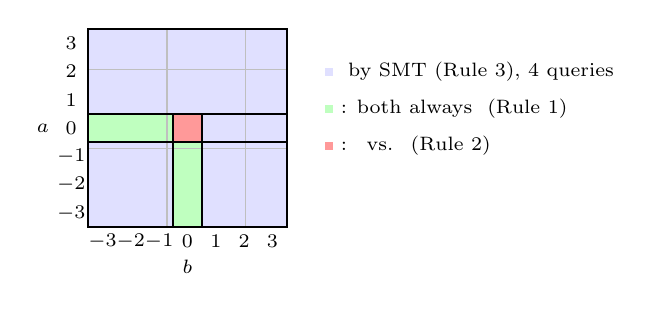
\begin{tikzpicture}[x=0.36cm, y=0.36cm, font=\scriptsize]
    \def\cell#1#2#3{\fill[#3] (#1,#2) rectangle ++(1,1);}
    % b on x-axis (-3..3 -> 0..6), a on y-axis (-3..3 -> 0..6)
    \fill[blue!12] (0,0) rectangle (3,3);   % a<0, b<0: SMT
    \fill[blue!12] (4,0) rectangle (7,3);   % a<0, b>0: SMT
    \fill[green!25] (3,0) rectangle (4,3);  % a<0, b=0: rule 1
    \fill[green!25] (0,3) rectangle (3,4);  % a=0, b<0: rule 1
    \fill[red!40]   (3,3) rectangle (4,4);  % (0,0): rule 2
    \fill[blue!12] (4,3) rectangle (7,4);   % a=0, b>0: SMT
    \fill[blue!12] (0,4) rectangle (7,7);   % a>0: SMT
    \draw[gray!50] (0,0) grid (7,7);
    \draw[thick] (0,0) rectangle (7,7);
    \draw[thick] (0,4) -- (7,4) (0,3) -- (7,3);
    \draw[thick] (3,0) -- (3,4) (4,0) -- (4,4);
    \foreach \v [count=\i from 0] in {-3,...,3} {
      \node at (\i+0.5,-0.5) {$\v$};
      \node at (-0.6,\i+0.5) {$\v$};
    }
    \node at (3.5,-1.4) {$b$};
    \node at (-1.6,3.5) {$a$};
    \node[anchor=west, align=left] at (8,5.5) {\tikz\fill[blue!12] (0,0) rectangle (0.3,0.3); \pres{} by SMT (Rule 3), 4 queries};
    \node[anchor=west, align=left] at (8,4.2) {\tikz\fill[green!25] (0,0) rectangle (0.3,0.3); \pres{}: both always \dbz{} (Rule 1)};
    \node[anchor=west, align=left] at (8,2.9) {\tikz\fill[red!40] (0,0) rectangle (0.3,0.3); \chg{}: \ok{} vs.\ \dbz{} (Rule 2)};
  \end{tikzpicture}
  \caption{Regions decided by the hybrid checker for \code{ratio} on $[-3,3]^2$. Thick lines
  are region borders; every input lies in a region with a proved verdict.}
  \label{fig:ratio}
\end{figure}

\paragraph{A value-only change}
The second kind of edit our approach targets is one where both versions always finish
normally. The corpus pair \code{sign} computes the sign of \code{x} with
\code{if (x > 0) return 1; if (x < 0) return -1; return 0;}. The edit deletes the second
test, so the method ends in \code{return -1}, and at $x = 0$ it returns $-1$ instead of
$0$. Both versions have outcome set $\set{\ok}$ and return interval $[-1,1]$ on every
domain, so no outcome-based analysis can see the change: the difference lies in the
\emph{relation} between input and output. On the whole domain the return query finds the
witness $x = 0$, which replays (Rule~3$'$). That proves the change but certifies one input,
so the checker keeps splitting at the constants of the code. On the point region
$x \in [0,0]$ the return intervals are $[0,0]$ and $[-1,-1]$, which are disjoint, so that
region is \chg{} (Rule~2b). On the regions below and above $0$ both versions return the
same constant, $-1$ or $1$, so those regions are \pres{} (Rule~2b$'$). One input is
\chg{}, the other six are \pres{}, and coverage is 100\%. Even without the solver the
splitting alone reaches the same map.

\section{Approach}
\label{sec:approach}

\begin{figure}
  \centering
  \begin{tikzpicture}[font=\footnotesize, node distance=5mm and 7mm,
      box/.style={draw, rounded corners=2pt, align=center, minimum height=9mm, inner sep=3pt},
      dec/.style={draw, diamond, aspect=2, align=center, inner sep=0.5pt},
      res/.style={draw, rounded corners=2pt, align=center, fill=gray!12, minimum height=9mm, inner sep=3pt},
      >={Stealth[length=2mm]}]
    % top row
    \node[box] (in) {pair $(A,B)$\\ domain $D$};
    \node[box, right=of in] (q) {queue of\\ regions};
    \node[box, right=of q] (ai) {interval analysis\\ $\hat A(R)$, $\hat B(R)$};
    \node[dec, right=of ai] (rules) {Rules\\ 0--2b$'$};
    \node[res, right=9mm of rules] (dec1) {region\\ decided};
    \node[res, right=of dec1] (out) {region map,\\ verdict,\\ coverage};
    % bottom row
    \node[dec, below=9mm of rules] (both) {both\\ $\set{\ok}$?};
    \node[box, right=9mm of both] (smt) {Z3 bit-vector\\ return query};
    \node[box, below=9mm of ai] (replay) {replay witness,\\ keep it};
    \node[box, below=9mm of q] (split) {split $R$ at\\ code constants};
    % edges
    \draw[->] (in) -- (q);
    \draw[->] (q) -- node[above]{$R$} (ai);
    \draw[->] (ai) -- (rules);
    \draw[->] (rules) -- node[above]{yes} (dec1);
    \draw[->] (dec1) -- (out);
    \draw[->] (rules) -- node[right]{no} (both);
    \draw[->] (both) -- node[above]{yes} (smt);
    \draw[->] (smt) -- node[right]{UNSAT} (dec1);
    \draw[->] (smt.south) -- ++(0,-0.45) -| node[pos=0.2, below]{SAT} (replay.south);
    \draw[->] (both) -- node[above]{no} (replay.east |- both) ;
    \draw[->] (replay) -- (split);
    \draw[->] (split) -- (q);
  \end{tikzpicture}
  \caption{Overview. The verdict rules decide a region from the interval analyses of both
  versions; only regions where both provably return normally reach the solver. Undecided
  regions, and regions with a replayed witness, are split until a region budget is reached.}
  \label{fig:overview}
\end{figure}

\Cref{fig:overview} gives an overview. We first define what we mean by the same behaviour
(\cref{sec:background}). We then describe the analysis, the verdict rules and the refinement
loop (\cref{sec:formal}). Finally we state their guarantees (\cref{sec:guarantees}).

\subsection{Background}
\label{sec:background}

\paragraph{Observations}
A \emph{pair} is two static methods $A$ and $B$ with the same descriptor. We support methods
with \code{int} parameters, an \code{int} or \code{void} result, and only integer
instructions, branches, \code{goto} and the assertion pattern. Calls, the heap and
\code{try}/\code{catch} make a pair unsupported. An input is a vector
$x \in \mathbb{Z}_{32}^n$. Running $P$ on $x$ yields the \emph{observation}
$\mathit{obs}_P(x) = (o, v)$. Here $o$ is the outcome class (\ok{}, \code{assertion error},
\dbz{}, \code{*} for non-termination, \ldots). The value $v$ is the 32-bit return value if
$o = \ok{}$, and $\bot$ otherwise. We do not observe exception messages, timing or the path
taken. $A$ and $B$ \emph{agree on $x$} iff $\mathit{obs}_A(x) = \mathit{obs}_B(x)$. A
region $R = I_1 \times \dots \times I_n$ is a box of integer intervals. The pair is
\emph{preserved on $R$} if it agrees on every $x \in R$. It is \emph{changed on $R$} if it
disagrees on some $x \in R$. Supported methods are deterministic, so $\mathit{obs}_P$ is a
function.

\paragraph{Interval abstract interpretation}
Abstract interpretation~\citep{cousot1977abstract} runs a program on abstract values that
each describe a set of concrete values. We use the interval lattice over Java \code{int}s,
$\mathcal{I} = \set{[l,u] \mid \mathit{MIN} \le l \le u \le \mathit{MAX}} \cup \set{\bot}$,
ordered by inclusion. The concretisation is $\gamma([l,u]) = \set{v \mid l \le v \le u}$ and
the abstraction is $\alpha(S) = [\min S, \max S]$. This pair is a Galois connection. An
abstract operation $\mathit{op}^\sharp$ is sound if two conditions hold. First,
$\mathit{op}(x,y) \in \gamma(\mathit{op}^\sharp(X,Y))$ for all $x \in \gamma(X)$ and
$y \in \gamma(Y)$ on which $\mathit{op}$ does not throw. Second, its error set contains every
exception that $\mathit{op}$ can raise there. The lattice has height about $2^{32}$, so loops
need a widening operator $\nabla$ to reach a fixpoint quickly.

\paragraph{Symbolic execution and SMT}
Symbolic execution~\citep{king1976symbolic} runs a program on symbolic inputs. For each
feasible path $\pi$ it collects a path condition and a symbolic result. We can compare two
loop-free methods by asking an SMT solver whether some input satisfies a path condition of
each version and makes the results differ. Java \code{int} arithmetic wraps, so we use 32-bit
bit-vectors. Their \code{bvsdiv} and \code{bvsrem} match \code{idiv} and \code{irem},
including $\mathit{MIN} / {-1} = \mathit{MIN}$. Unbounded integers give wrong answers near the
limits.

\subsection{Formal Description}
\label{sec:formal}

\paragraph{Region analysis}
For a version $P$ and a non-empty region $R$, the analysis computes an outcome set
$\hat P(R)$ and a return interval $\hat r_P(R)$. It is a forward worklist interpreter
over bytecode offsets. The abstract state at each offset is a tuple of intervals for the
locals and a stack of values. The initial state maps parameter $i$ to $I_i$. The analysis has
four parts.
\begin{itemize}
  \item \emph{Arithmetic.} $+$, $-$ and $\times$ compute the mathematical bounds and return
        $\top$ if a bound leaves the \code{int} range. Negation works the same way. For
        $X / Y$ and $X \,\%\, Y$ we add \dbz{} iff $0 \in Y$. We compute the result
        separately on the negative and the positive part of $Y \setminus \set{0}$, and we join
        the two results (\cref{thm:intervals}).
  \item \emph{Branch refinement.} We follow a conditional branch on $X \bowtie Y$ on each
        side, with $X$ and $Y$ narrowed by the condition or its negation. An empty interval
        marks the side as infeasible. Narrowing a stack value is not enough. Every stack value
        therefore carries a tag $\mathit{src}$ that names the local it was loaded from. The
        tag is cleared when that local is written, and we narrow the local itself too. This is
        how $b \neq 0$ in \code{if (b == 0) return 0} reaches the later division. Intervals
        cannot express a hole, so $\neq$ only removes an endpoint.
  \item \emph{Loops.} At a backward edge we widen the new state. An interval bound that grew
        jumps to $\mathit{MIN}$ or $\mathit{MAX}$. Every reachable backward edge adds the
        outcome \code{*} (``may not terminate''), unless the loop matches the counting pattern
        that \code{javac} emits for \code{for (i = ..; i < n; i++)}. That pattern has a single
        exit test \code{i >= n}, a straight-line body with exactly one \code{i += 1}, and no
        writes to \code{i} or \code{n}. Such a loop always exits. The code also accepts the
        mirrored decreasing counter, but we prove only the increasing case.
  \item \emph{Unsupported code.} Any other instruction makes the result \emph{unsupported},
        with the full outcome set and $\top$ returns. No rule can then fire.
\end{itemize}

\paragraph{Verdict rules}
For a region $R$ we try the rules below in order. The first rule that matches decides.
\begin{center}
\small
\begin{tabular}{@{}llll@{}} \toprule
\# & Condition & Verdict & Scope \\ \midrule
0  & $\hat A(R) = \emptyset$ or $\hat B(R) = \emptyset$ & \unk{} & analysis failure \\
1  & $\hat A(R) = \hat B(R) = \set{e}$, $e \neq \ok$ & \pres{} & all of $R$ \\
2  & $\hat A(R) \cap \hat B(R) = \emptyset$ & \chg{} & all of $R$ \\
2b & both $\set{\ok}$, $\hat r_A(R) \cap \hat r_B(R) = \emptyset$ & \chg{} & all of $R$ \\
2b$'$ & both $\set{\ok}$, $\hat r_A(R) = \hat r_B(R) = [c,c]$ & \pres{} & all of $R$ \\
3  & both $\set{\ok}$ and $\Phi(R)$ UNSAT & \pres{} & all of $R$ \\
3$'$ & both $\set{\ok}$ and $\Phi(R)$ has a model $w$ that replays & \chg{} & witness $w$ only \\
4  & otherwise & \unk{}, split $R$ & \\ \bottomrule
\end{tabular}
\end{center}
Rule~1 needs a \emph{singleton} set. Equal sets with two outcomes prove nothing. In
\cref{lst:example} both sets are $\set{\ok, \dbz}$ on $D$, yet the versions differ at
$(0,0)$. In general $A$ and $B$ may swap their outcomes between inputs.

\paragraph{Return comparison}
For rules 3 and 3$'$ we execute both versions symbolically over \emph{shared} bit-vector
inputs $\vec x$. We collect their normally returning paths $(\pi_{P,i}, r_{P,i})$. Every
division on such a path adds the condition ``divisor $\neq 0$'' to $\pi$. SMT-LIB defines
$x / 0$, while Java throws. Then
\[
  \Phi(R) \;=\; \vec x \in R \;\wedge\; \bigvee_{i,j}\bigl(\pi_{A,i} \wedge \pi_{B,j}
  \wedge r_{A,i} \neq r_{B,j}\bigr).
\]
Before we trust an UNSAT answer, we ask Z3 whether the collected paths cover all of $R$ for
both versions. If they do not, the answer is \unk{}. We replay a model $w$ on an independent
concrete interpreter with Java \code{int} semantics. We report it only if the two observations
really differ. A solver timeout, a backward jump or more than 256 paths also give \unk{},
never \pres{}.

\paragraph{Refinement}
\code{check\_pair} keeps a queue of regions, starting with $D$. We split an undecided region
with \code{split\_region}. We take the first parameter whose interval strictly contains a
constant $c$ pushed by either version (or $0$). The split produces $[l, c-1]$, $[c,c]$ and
$[c+1, u]$. Without such a constant we bisect the widest interval. The children are disjoint
and cover the parent. A region decided by Rule~3$'$ keeps its witness but is still split, so
we can certify the rest of it. A budget of about 200 regions bounds the loop. Regions left over
stay \unk{}. The pair verdict is \chg{} if any witness exists, \pres{} if \pres{} regions
cover $D$, and \unk{} otherwise. The \emph{certified coverage} is the fraction of $D$ in
\pres{} regions, whole-region \chg{} regions and witness points.

\subsection{Theoretical Guarantees}
\label{sec:guarantees}

The checker rests on two abstractions. The \emph{interval abstraction} abstracts sets of
\code{int} values. The \emph{region abstraction} abstracts the observation function of a
version on a box. It maps $\mathit{obs}_P$ restricted to $R$ to the pair
$(\hat P(R), \hat r_P(R))$. Its concretisation is
$\gamma(O, r) = \set{(o, v) \mid o \in O,\; o = \ok \Rightarrow v \in \gamma(r)}$. We prove
both abstractions sound and prove that widening terminates. We then derive the correctness of
the verdicts.

\begin{theorem}[Interval transfer functions]
\label{thm:intervals}
Each abstract operation $+^\sharp, -^\sharp, \times^\sharp, /^\sharp, \%^\sharp$ and
$-^\sharp$ (negation) satisfies the soundness condition of \cref{sec:background}, and
$/^\sharp$ and $\%^\sharp$ report \dbz{} iff $0 \in Y$.
\end{theorem}
\begin{proof}
Let $X = [a,b]$ and $Y = [c,d]$. For $+$, $-$ and $\times$, the bounds of the mathematical
result over the box $X \times Y$ lie at its corners. The operations $+$ and $-$ are monotone in
each argument, and $\times$ is linear in each argument. If both bounds lie in the \code{int}
range, every Java result equals the mathematical one. Otherwise the result is $\top$, which
contains every wrapped value. Negation is the case $[-b,-a]$, and only $-\mathit{MIN}$ wraps.
For division, \code{idiv} throws iff $y = 0$. So ``\dbz{} iff $0 \in Y$'' is exact in both
directions. Only $y \in Y \setminus \set{0}$ reaches the quotient. This set is the union of a
negative and a positive interval, so it suffices to bound each part and join. On a part with
fixed sign, $q(x,y) = \mathit{trunc}(x/y)$ is monotone in $x$ for fixed $y$. For fixed $x$ it
attains its extreme over $y$ at an endpoint. The four corners therefore bound it. Since
$|q| \le |x|$, only $\mathit{MIN}/{-1}$ can overflow, and that case returns $\top$. For
remainder, Java guarantees three facts. The result $x \,\%\, y$ is $0$ or has the sign of $x$.
We have $|x \,\%\, y| \le |y| - 1$. We also have $|x \,\%\, y| \le |x|$. With
$m = \max(|c|,|d|) - 1$ on a part, these facts give the bounds
$[\,0 \text{ or } \max(a,-m),\; 0 \text{ or } \min(b,m)\,]$ that we compute.
\end{proof}

\begin{lemma}[Branch refinement]
\label{lem:refine}
For every $x \in X$, $y \in Y$ with $(x \bowtie y) = h$, the refined intervals
$(X', Y')$ contain $x$ and $y$.
\end{lemma}
\begin{proof}
The case $h = \mathit{false}$ uses the negated condition. On integers this is again one of
$=, \neq, <, \le, >, \ge$. For each condition the bounds follow directly. For example,
$x < y \le d$ implies $x \le d - 1$, and $y > x \ge a$ implies $y \ge a + 1$. For $=$ both
values lie in $X \cap Y$. For $\neq$ we remove a value $v$ from $X$ only when $Y = [v,v]$ and
$v$ is an endpoint of $X$. Narrowing the local named by the $\mathit{src}$ tag is sound. A load
sets the tag, and every write to that local clears it. The tag therefore holds only while the
stack value equals the current content of the local.
\end{proof}

\begin{theorem}[Widening terminates]
\label{thm:widening}
$X \sqsubseteq X \nabla Y$ and $Y \sqsubseteq X \nabla Y$, and every chain
$X_0, X_1 = X_0 \nabla Y_1, X_2 = X_1 \nabla Y_2, \ldots$ is eventually constant.
\end{theorem}
\begin{proof}
$X \nabla Y$ keeps each bound of $X$ that $Y$ does not exceed. It moves the other bound to
$\mathit{MIN}$ or $\mathit{MAX}$. The result therefore contains both arguments. Along a chain
each of the two bounds changes at most once, from its current value to its limit, and it
cannot grow after that. A chain therefore changes at most twice. With $k$ locals and stack
slots at a loop head, the abstract state there changes at most $2k$ times. The worklist
revisits a program point only when its state grows, so it terminates.
\end{proof}

\begin{theorem}[Soundness of the region analysis]
\label{thm:region}
For every supported $P$, non-empty region $R$ and $x \in R$:
$\mathit{out}_P(x) \in \hat P(R)$, and $\mathit{ret}_P(x) \in \gamma(\hat r_P(R))$ if
$\mathit{out}_P(x) = \ok$. We call this property (S).
\end{theorem}
\begin{proof}
We show an invariant. Every concrete state $(\mathit{pc}, \mathit{locals}, \mathit{stack})$
reached from an input in $R$ lies in the concretisation of the abstract state stored at
$\mathit{pc}$, interval by interval. The invariant holds initially, because parameter $i$
starts in $I_i$. Each instruction preserves it by \cref{thm:intervals} and \cref{lem:refine}.
Joins and widenings only enlarge states (\cref{thm:widening}). At the fixpoint the invariant
covers every reachable state. Each concrete step that ends the method is matched by an
abstract step. A \code{return} adds \ok{} and joins the returned interval into $\hat r_P$. A
division adds \dbz{} whenever its divisor may be $0$. Constructing an \code{AssertionError}
adds \code{assertion error}. We reject methods with exception handlers, so every exception
escapes. A non-terminating execution must follow some backward edge infinitely often. The
analysis adds \code{*} for every reachable backward edge except a counting loop. Such a loop
runs its body only while $i < n \le \mathit{MAX}$. So $i + 1$ cannot wrap, and $n - i$
decreases by one in every iteration. We reject the pattern \code{i <= n}, because with
$n = \mathit{MAX}$ it never exits.
\end{proof}

\paragraph{Soundness of the verdicts}
With (S), the verdict rules are correct.
\begin{itemize}
  \item \emph{Rule 1.} By (S), both versions end in $e$ on every $x \in R$. Error observations
        carry no value, so $\mathit{obs}_A(x) = (e,\bot) = \mathit{obs}_B(x)$.
  \item \emph{Rule 2.} By (S), $\mathit{out}_A(x) \in \hat A(R)$ and
        $\mathit{out}_B(x) \in \hat B(R)$. The sets are disjoint, so the outcomes differ for
        every $x$. Rule~0 must run first, because an empty set would make Rule~2 fire
        vacuously.
  \item \emph{Rules 2b and 2b$'$.} These are the same arguments applied to the return
        intervals. We treat an empty return interval like Rule~0.
  \item \emph{Rule 3.} Suppose the versions disagree on some $x \in R$. Both return normally,
        so $\mathit{ret}_A(x) \neq \mathit{ret}_B(x)$. The paths are complete, which we check,
        and execution is deterministic. So $x$ satisfies exactly one $\pi_{A,i}$ and one
        $\pi_{B,j}$, and then $x$ is a model of $\Phi(R)$. This contradicts UNSAT. The proof
        needs the bit-vector encoding, the divisor conditions and the shared inputs.
  \item \emph{Rule 3$'$.} A replayed witness is a concrete disagreement.
\end{itemize}
Refinement terminates, because every split strictly shrinks a finite region and the budget
bounds the number of regions. The children partition their parent, so coverage counts each
input once. Hence a \pres{} verdict is a proof over all of $D$. A \chg{} verdict always comes
with a witness, either a replayed solver model or a point of a region that differs everywhere.
The checker is not complete. Intervals cannot relate two variables, so non-constant return
values need the solver. Loops with loop-dependent return values stay \unk{}. Besides the
proofs, we checked every interval operation with property-based tests and with brute-force
checks on intervals with endpoints near $0$, $\mathit{MIN}$ and $\mathit{MAX}$.

\section{Evaluation}
\label{sec:evaluation}

We split the research question into three sub-questions.
\begin{description}
  \item[RQ1 (soundness)] Does the checker ever give a wrong verdict in practice?
  \item[RQ2 (coverage)] How much of the input domain does it certify, compared with one SMT
        query over the whole domain and with differential testing?
  \item[RQ3 (layers)] What does each layer contribute? What do the intervals add on top of
        the solver, and the solver on top of the intervals, and at what cost?
\end{description}

\subsection{Setup}
\label{sec:setup}

\paragraph{Benchmarks}
We use 20 method pairs in three groups. The \emph{corpus} (\code{Refactorings.java}) holds 10
pairs that we wrote for this project. Five are preserving edits: inlining a temporary,
removing dead code, inverting a branch, reversing a \code{max} comparison, and an unchanged
pair. Three are value-only faults: \code{sign}, \code{absVal} and an off-by-one comparison
\code{belowTwo}. Two are exception faults: guard removals in \code{ratio} and
\code{reciprocal}. For the corpus, ground truth comes from the real JVM. A Java harness runs
both versions with \code{-ea} on all 238 inputs of the declared domains and records outcome
and return value. Five pairs
come from the stock \jpamb{} class \code{Simple}. Two of them compare a method with itself and
act as controls. Five evaluation-only pairs (\code{EvalPairs.java}) contain loops or many
paths. The loop pairs are \code{loopDiv} with an added guard, \code{loopDiv} with a rewritten
body, and \code{loopThenZero}. The many-path pairs are two versions of \code{ladder}, which has
twelve sequential \code{if} statements. One version reorders them and the other changes one
constant.

\paragraph{Configurations}
We compare four configurations on each pair.
\begin{itemize}
  \item \code{gate}: intervals, verdict rules 0 to 2b$'$ and refinement, without the solver.
  \item \code{hybrid}: our full approach.
  \item \code{z3only}: one SMT query over the whole domain. It encodes both the error paths
        and the returning paths, so it compares outcome class and value together. This is a
        baseline in the style of differential symbolic execution~\citep{person2008dse},
        without the interval layer.
  \item \code{random}: differential testing~\citep{mckeeman1998differential} with 1000
        uniformly random inputs (seed 0) on a concrete interpreter with Java \code{int}
        semantics. Without a difference it answers \unk{} and never \pres{}.
\end{itemize}
We run every pair on a \emph{small} domain $[-3,3]^k$ and on a \emph{large} domain
$[-1000,1000]^k$, which has up to 4 million inputs. On the small domain ground truth comes
from exhaustive execution. On the large domain we check a \pres{} verdict against 2000 random
inputs. We replay solver witnesses (Rule~3$'$). We do not replay whole-region \chg{} verdicts.

\paragraph{Metrics}
A verdict is \emph{wrong} if it says \pres{} while a difference exists, or \chg{} without a
real difference. An \unk{} verdict is never wrong. A pair is \emph{decided} if the verdict is
not \unk{}. The \emph{certified coverage} is the fraction of the domain with a proved verdict
(\cref{sec:formal}). For the baselines it is $1$ for \pres{} and one input for a witness.

\paragraph{Environment}
We use Python~3.13, the \jpamb{} 0.9.0 bytecode model and Z3 5.4.1, with a 5\,s timeout per
SMT query and a region budget of about 200. We run on a laptop (Intel Core i5-1038NG7, 16\,GB,
macOS). The times come from a single run. \Cref{app:variance} has repeated timings.

\subsection{Results}
\label{sec:results}

\begin{table}
  \centering
  \caption{Summary over 20 pairs per domain (40 runs per configuration). \emph{Coverage}
  is the mean certified coverage. \emph{SMT} is the number of solver queries in total.}
  \label{tab:results}
  \small
  \begin{tabular}{@{}l rrrr rrrr r@{}} \toprule
    & \multicolumn{4}{c}{small $[-3,3]^k$} & \multicolumn{4}{c}{large $[-1000,1000]^k$} & all \\
    \cmidrule(lr){2-5} \cmidrule(lr){6-9}
    Config & decided & coverage & SMT & ms & decided & coverage & SMT & ms & wrong \\ \midrule
    gate   & 19/20 & 98\% & 0   & 1014 & 13/20 & 61\% & 0   & 4418  & 0 \\
    hybrid & 19/20 & 98\% & 101 & 1120 & \textbf{19/20} & \textbf{95\%} & 566 & 6396 & 0 \\
    z3only & 17/20 & 49\% & 20  & 1082 & 17/20 & 40\% & 20  & 1265  & 0 \\
    random & 9/20  & 5\%  & 0   & 1165 & 9/20  & $<$1\% & 0 & 35422 & 0 \\ \bottomrule
  \end{tabular}
\end{table}

\Cref{tab:results} summarises the 160 runs. \Cref{tab:perpair} in \cref{app:perpair} lists
every pair.

\paragraph{RQ1: Soundness}
No configuration produced a wrong verdict. We checked each pair against exhaustive execution
on the small domain and against 2000 samples on the large one. Solver witnesses replay by
construction, because we report a model that does not replay as \unk{}. The pair harness, with a
matched 5\,s budget per pair, passes all 10 corpus pairs for both the analyser and seeded
differential testing. The pair \code{ladder/\_changed} shows that a verdict holds only for its
domain. The edit changes a constant that lies outside $[-3,3]$. The pair is therefore \pres{}
on the small domain and \chg{} on the large one. All four configurations agree with that.

\paragraph{RQ2: Coverage}
On the large domain the hybrid decides 19 of 20 pairs and certifies 95\% of the inputs on
average. One SMT query over the domain decides 17 of 20 and certifies 40\%. Random testing
decides 9 of 20 and certifies under 1\%. The gap in coverage comes from the \chg{} pairs. The
\code{z3only} and \code{random} configurations certify only their witness. The hybrid also
proves the rest of the domain. For \code{ratio} it proves 48 of 49 inputs \pres{} on the small
domain. On the large domain it proves all but the one input $(0,0)$ of four million. Random
testing finds this input in none of 20 seeds (\cref{app:variance}).

\paragraph{RQ3: Loops}
The symbolic executor rejects backward jumps, so \code{z3only} answers \unk{} on all three
loop pairs. The interval layer still decides two of them. Both versions of
\code{loopThenZero} end in \code{s / 0} after a counting loop that provably terminates. Their
outcome set is $\set{\dbz}$, and Rule~1 proves the pair \pres{} on the whole domain in one
region analysis. For \code{loopDiv} with an added guard, we split at $d = 0$. This isolates a
region with disjoint outcome sets, which gives a whole-region \chg{} verdict. It certifies
76\% (small) and 50\% (large) of the inputs.

\paragraph{RQ3: Cost}
On loop-free pairs one SMT query is the fastest way to a verdict. The \code{z3only}
configuration needs 1.3\,s for all large-domain runs, and the hybrid needs 6.4\,s. The extra
time buys coverage. After the hybrid finds a witness, it keeps splitting and querying. This
costs most in time on \code{justAdd/justMulitply} (144 queries, 2.7\,s) and on
\code{ladder/\_changed}. The two \code{loopDiv} pairs issue 190 queries each that fail at once
on loops.

\subsection{Discussion}
\label{sec:discussion}

On these 20 small, \code{int}-only pairs the answer to the research question is yes, with a
qualification. No verdict was wrong on any run. The hybrid is the only configuration that
both decides most pairs and says where an edit changes behaviour. The two layers complement
each other. The intervals decide regions where the outcome classes differ or coincide on a
single error, and they handle loops. The solver decides regions where both versions return and
only the value is in question. Alone, each layer falls short. Without the solver, the gate
decides none of the five preserving corpus pairs on the large domain, because intervals cannot
relate the two versions. Without the gate, \code{z3only} cannot handle loops and certifies no
more than a witness. The qualification is that \code{z3only} is the faster way to a yes or no
verdict on loop-free code. The many-path pairs caused no path explosion, so we make no claim
about scalability in the number of paths. The pair \code{loopDiv/\_rewritten} stays \unk{}
everywhere. Both versions return a loop-dependent value that neither layer can relate.

\subsection{Threats to Validity}
\label{sec:threats}

\paragraph{Internal}
Coverage favours methods that localise, because \code{z3only} stops at one witness. We
therefore treat decided runs as the primary measure. We wrote the corpus and the extra pairs
ourselves. The splitting heuristic uses the constants that appear in the code, which suits
small hand-written pairs. We reduce the risk of bugs in the checker in three ways. We take the
corpus ground truth from the real JVM, we replay solver witnesses, and we test the interval
operations against Java semantics with property-based tests. For the \code{Simple} and
\code{EvalPairs} groups the ground truth comes from our Python interpreter. We tested that
interpreter against the real-JVM observations, but only on the corpus. On the large domain we
only spot-check a \pres{} verdict by sampling, so a soundness bug that affects few inputs could
go unnoticed there. We did not mechanise the proofs in \cref{sec:guarantees}. Code review found
one gap between proof and code. Exception tables were ignored, so a caught division gave a
false \chg{} verdict. We now reject methods with handlers. Soundness assumes \code{-ea} and
\code{javac}-shaped loops. A 10,000-step cap gives \emph{unsupported}.

\paragraph{External}
The 20 pairs are small, static, \code{int}-only and call-free. The domains are boxes of at
most $2001^2$ inputs. Real refactorings involve objects, calls and caught exceptions, which our
observation contract excludes. The results say nothing about them. A verdict holds only on the
declared domain, not on all of \code{int}.

\section{Related Work}
\label{sec:related}

\paragraph{Regression verification and equivalence checking}
\citet{godlin2009regression} introduced \emph{regression verification}: proving that two
closely related programs produce the same output for every input. They do it by pairing
recursive calls and checking loop-free bodies with a bounded model checker.
SymDiff~\citep{lahiri2012symdiff} translates both versions to an intermediate verification
language and checks equivalence with an SMT solver, reporting a counterexample when the
versions differ. Both give one verdict for the whole input space. Our Rule~3 is such a
check, but we only ask it on regions where the interval layer has already shown that both
versions return normally, so the rest of the domain still receives a verdict.

\paragraph{Differential symbolic execution and partitioning}
Differential symbolic execution~\citep{person2008dse} summarises both versions symbolically
and abstracts unchanged code with uninterpreted functions. ARDiff~\citep{badihi2020ardiff}
refines those uninterpreted functions on demand when the abstraction is too coarse to decide
equivalence. Our z3only baseline is plainer: whole-method SMT equivalence with no abstraction of common code. Partition-based regression
verification~\citep{boehme2013prv} is the closest in spirit: it splits the input space into
partitions with the same symbolic paths, and reports each partition as equivalent or
different, so the result is useful even when the whole program cannot be decided.
PASDA~\citep{glock2024pasda} extends partition-based differencing with best-effort
classifications for partitions that cannot be proved. We share the goal of per-region
verdicts, but our partitions are boxes produced by splitting at code constants, and many of
them are decided by an abstract interpretation without path enumeration, which also
decides loop pairs such as \code{loopThenZero}.

\paragraph{Abstract interpretation of differences}
\citet{partush2013abstract} analyse the \emph{correlating program} of two versions with
numerical abstract domains, so that the abstraction can express relations such as
$x_A = x_B$ directly. \citet{trostanetski2017modular} compute under- and
over-approximations of the input sets on which two versions differ, procedure by procedure,
and refine summaries on demand. Partush and Yahav can express relations between the versions inside the abstract domain,
which helps on loops. We deliberately analyse each
version separately with plain intervals and leave relations to the solver, at the price of
the \unk{} for \code{loopDiv/\_rewritten}.

\paragraph{Alternatives from the course}
A \emph{syntactic analysis} (a bytecode diff, or patterns for known refactorings) cannot
tell that deleting \code{if (d == 0) return 0} matters only at $(0,0)$; we use syntax only
to collect the split constants. A \emph{bounded static analysis} silently drops long traces,
which breaks the soundness that Rules~1 and~2 need, so we use the unbounded analysis with
widening. \emph{Concolic execution} and \emph{coverage-guided fuzzing} would find better
witnesses than random testing, but like differential
testing~\citep{mckeeman1998differential} they can refute equivalence and never prove a
region \pres{}. A \emph{relational domain} such
as octagons~\citep{mine2006octagon} on a product program could prove some preserved loop
pairs, but needs a product construction and much harder soundness and widening proofs. We
chose intervals, whose proofs we could complete, and moved the relational reasoning to the
solver.

\section{Conclusion}
\label{sec:conclusion}

We asked whether an edit preserves the behaviour of a method, and where it does not. Our
checker splits the input domain into boxes. It decides each box with an interval analysis
of the two versions and sound verdict rules, and sends only the value comparison on boxes
where both versions return normally to a bit-vector SMT query. On 20 pairs and two domains
it never gave a wrong verdict. It decided 38 of 40 runs and certified 96\% of the inputs on
average, against 45\% for a single SMT query and 2\% for differential testing. It also
decided loop pairs that symbolic execution rejects. The main limitation is that intervals
cannot relate the two versions, so loops with loop-dependent results stay \unk{}. A
relational domain over a product program, and support for calls and the heap, are the
natural next steps.


% Appendix: does not count towards the 10 pages.
\appendix
\section{Data Availability}
\label{app:data}
% Where can the code, benchmarks and results be found? How do you reproduce them?

\todo{Link to repository and instructions to reproduce the results.}

\section{AI-Use Statement}
\label{app:ai}
% Which AI tools were used, for what (code, writing, research), and how the
% output was checked.

\todo{AI-use statement.}

\section{Technical Contributions}
\label{app:contributions}
% One row per technical contribution, using the codes from the project page.
% Points per contribution follow the formula on the project page (respect the max).
% Grade thresholds per student:
%   12: >=20 points across 5 contributions
%   10: >=15 points across 4 contributions
%    7: >=10 points across 3 contributions
%    4: >= 7 points across 3 contributions
%   02: >= 5 points across 3 contributions
% Note: PMG gives 0 points for a group of 3 (3 per person over 3).

\begin{table}[h]
  \centering
  \caption{Contributions. $S_1$ is Deniz Isikli (s215818), $S_2$ is Cristina Semikina (s260209), $S_3$ is Krish Devendra Waghresha (s252788).}
  \label{tab:contributions}
  \begin{tabular}{@{}llrrrr@{}} \toprule
    ID & Contribution & P & $S_1$ & $S_2$ & $S_3$ \\ \midrule
    \texttt{XXX} & Contribution & 0 & 0 & 0 & 0 \\
    \texttt{XXX} & Contribution & 0 & 0 & 0 & 0 \\
    \texttt{XXX} & Contribution & 0 & 0 & 0 & 0 \\
    \texttt{XXX} & Contribution & 0 & 0 & 0 & 0 \\
    \texttt{XXX} & Contribution & 0 & 0 & 0 & 0 \\
    \texttt{PWP} & Write Paper & 0 & 0 & 0 & 0 \\
    \texttt{PRW} & Read and relate to recent papers & 0 & 0 & 0 & 0 \\ \midrule
    \multicolumn{2}{l}{Total} & 0 & 0 & 0 & 0 \\
    \multicolumn{2}{l}{Suggested Max Grade} & - & - & - & - \\ \bottomrule
  \end{tabular}
\end{table}


\bibliographystyle{ACM-Reference-Format}
\bibliography{references}

\end{document}
